\section{APÉNDICES}

Los apéndices a continuación proporcionan material complementario que ofrece contexto visual a los requisitos funcionales detallados en la Sección 3.2.

\subsection{Diagramas de Modelado de Procesos (BPMN)}

Los siguientes diagramas fueron elaborados durante la fase de \textbf{Análisis de Procesos de Negocio (BPA)} y sirvieron como insumo principal para la elicitación y definición de los requisitos funcionales del sistema. Su propósito en este documento es ilustrar el flujo de trabajo (`workflow`) que las Historias de Usuario y los Requisitos Funcionales buscan automatizar y optimizar.

\subsubsection{Diagrama A: Ciclo de Mantenimiento Correctivo (Reactivo)}

Este diagrama modela el flujo completo desde la detección de una falla hasta el cierre administrativo de la Orden de Trabajo, evidenciando la interacción entre Técnicos, Supervisores y el Sistema.

\begin{figure}[H]
    \centering
    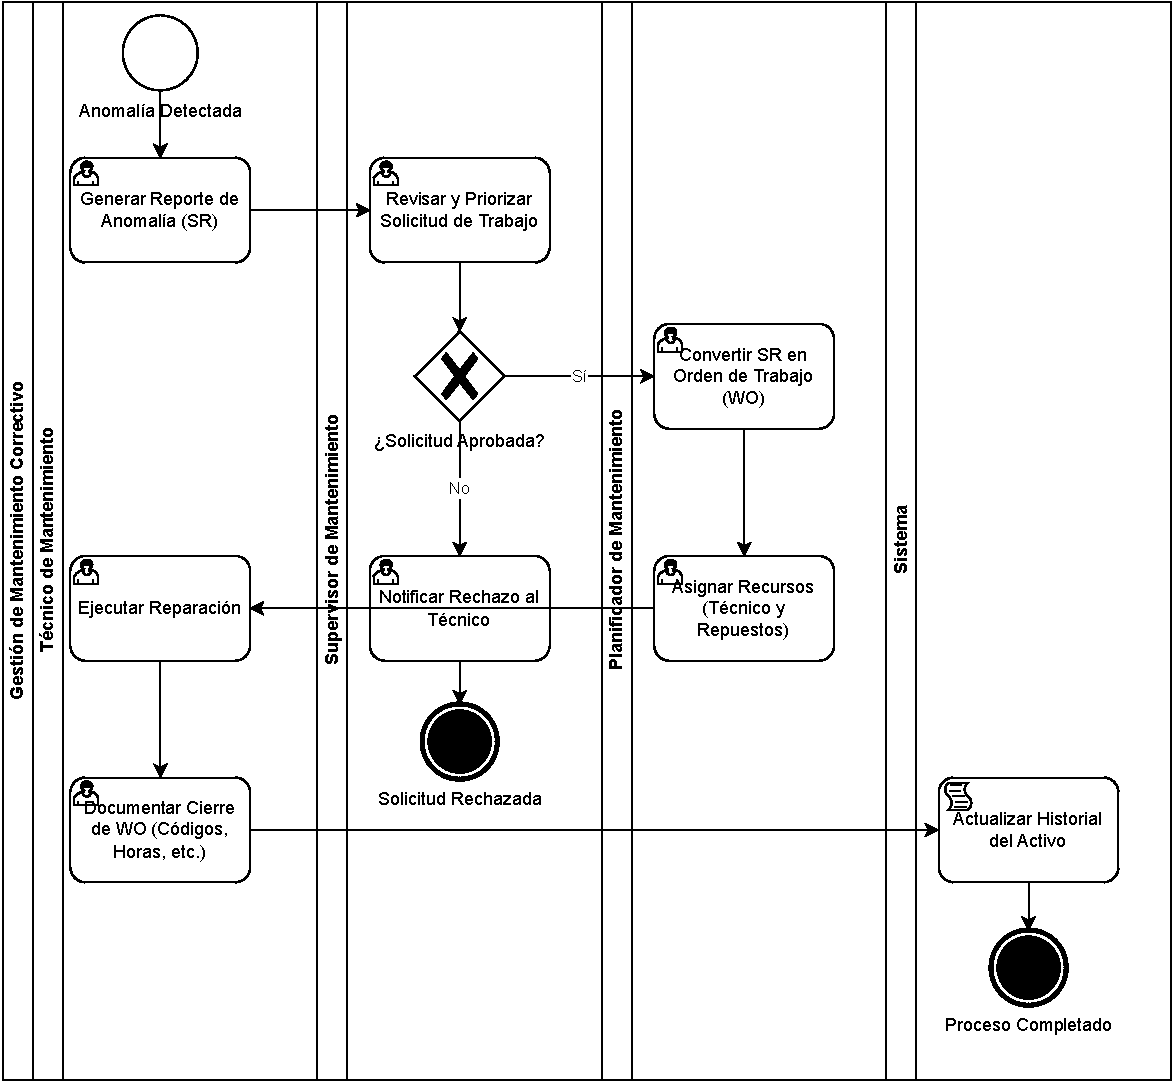
\includegraphics[width=0.95\textwidth]{assets/Diagrama_BPMN_CM.pdf}
    \caption{Diagrama A: Ciclo de Mantenimiento Correctivo}
\end{figure}

\subsubsection{Diagrama B: Ciclo de Mantenimiento Preventivo (Proactivo)}

Este flujo ilustra el proceso proactivo, donde el sistema genera y asigna automáticamente Órdenes de Trabajo basándose en un plan predefinido, optimizando la planificación y la ejecución.

\begin{figure}[H]
    \centering
    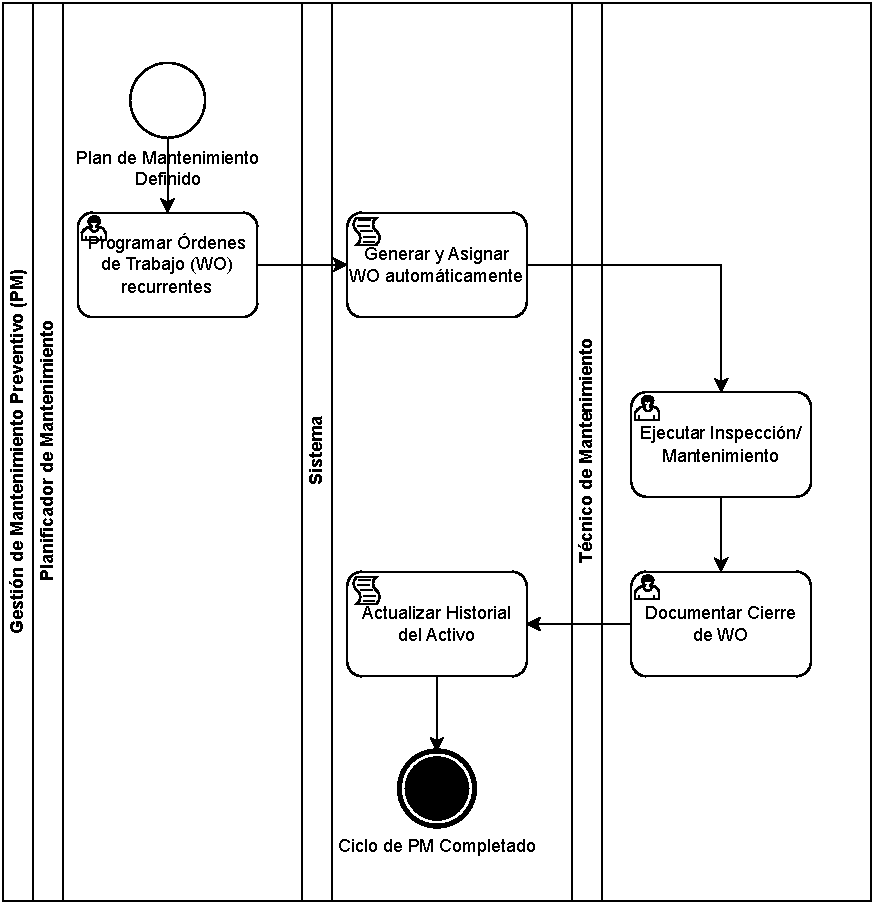
\includegraphics[width=0.95\textwidth]{assets/Diagrama_BPMN_PM.pdf}
    \caption{Diagrama B: Ciclo de Mantenimiento Preventivo}
\end{figure}

\subsubsection{Diagrama C: Ciclo de Mantenimiento Predictivo (Inteligente)}

Este modelo representa la estrategia más avanzada, mostrando cómo los datos de sensores son procesados por modelos de IA para generar alertas predictivas que anticipan fallas, permitiendo intervenciones justo a tiempo.

\begin{figure}[H]
    \centering
    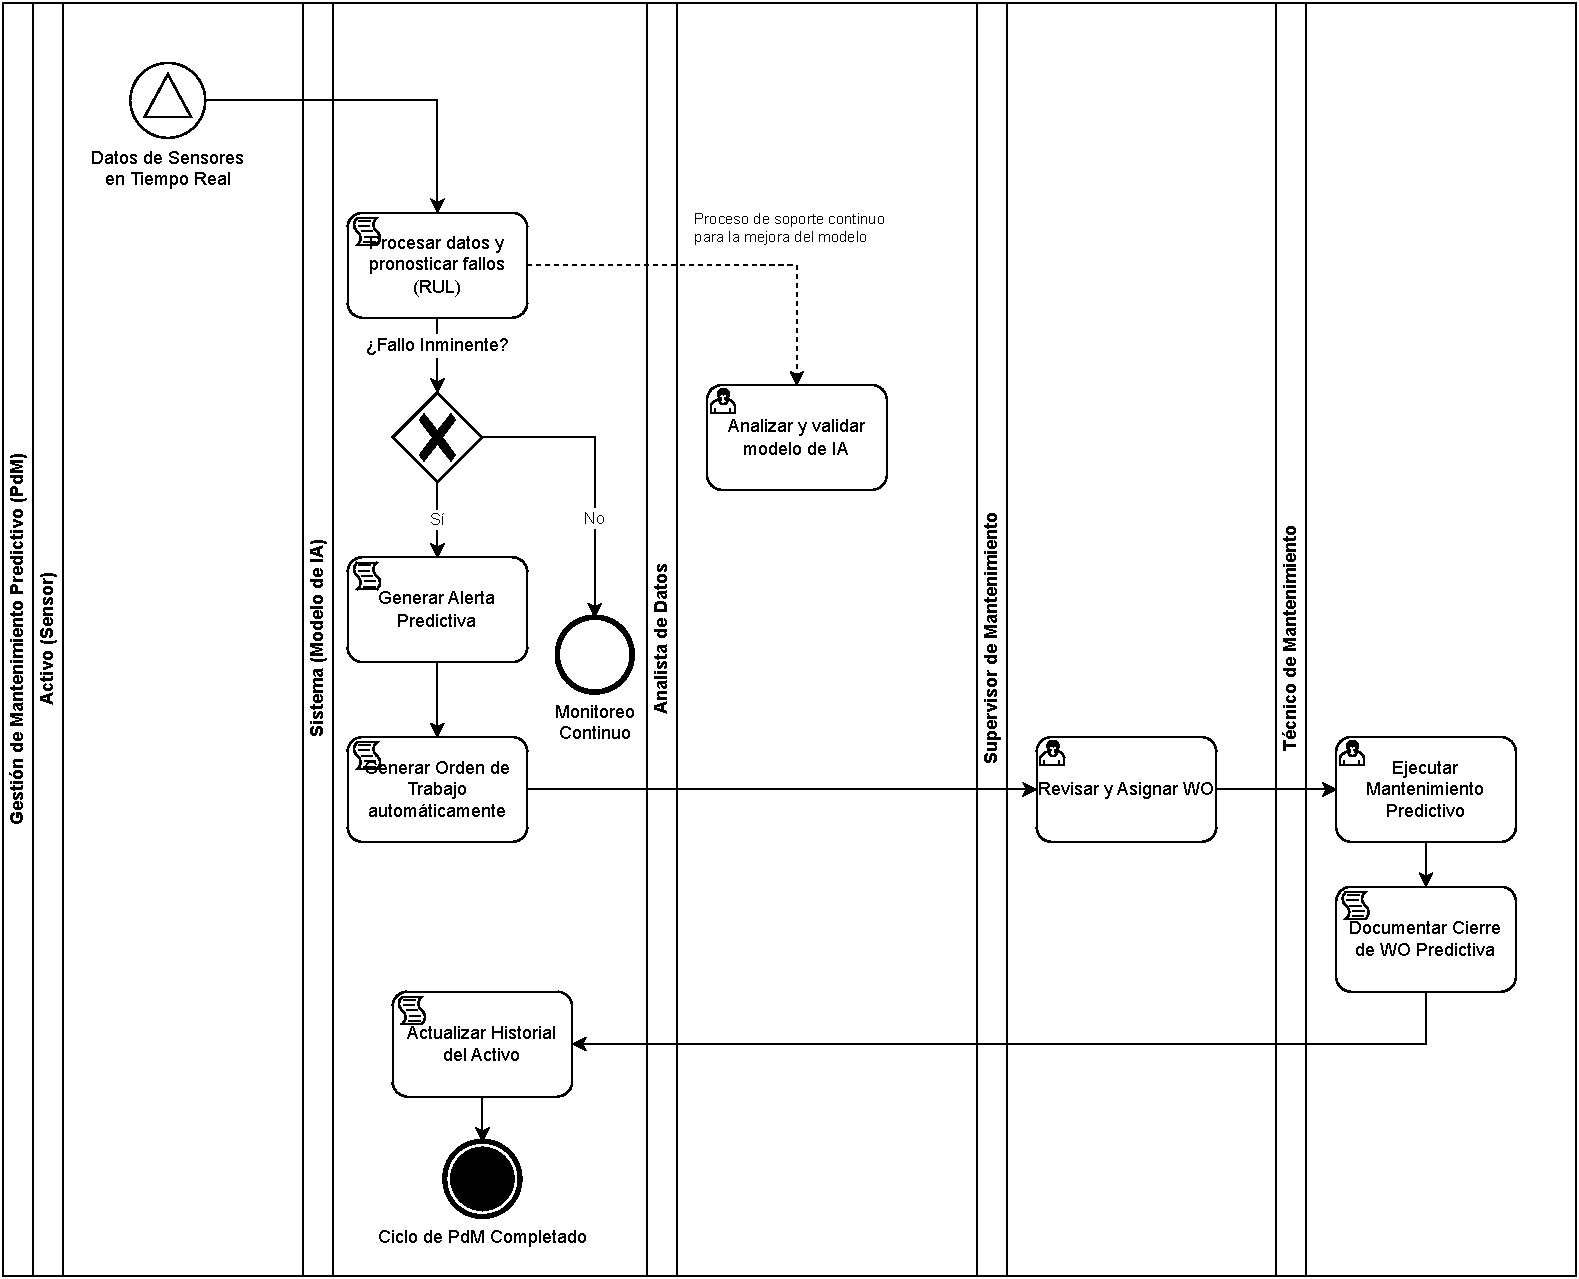
\includegraphics[width=0.95\textwidth]{assets/Diagrama_BPMN_PdM.pdf}
    \caption{Diagrama C: Ciclo de Mantenimiento Predictivo}
\end{figure}
